\documentclass[11pt,reqno,letter]{amsart}
%\pdfoutput=1
\usepackage{amsmath}

%----------------------------------------------------------------------------------------%

\usepackage{amsfonts}
\usepackage{amssymb}
\usepackage{amsthm}

\usepackage{graphicx}
\usepackage{hyperref}
\usepackage[left=1.25in,right=1.25in,top=1.5in,bottom=1.25in]{geometry}
\usepackage{multirow}
\usepackage{verbatim}
\usepackage{float}
\usepackage{rotating}
%\usepackage{pxfonts}
%\usepackage{isomath}
%\usepackage{newpxtext}
%\usepackage{newpxmath}
\usepackage[dvipsnames]{xcolor}
\usepackage[normalem]{ulem}
\usepackage{booktabs}


% packages for rmd output
\usepackage{tabu}
\providecommand{\tightlist}{%
  \setlength{\itemsep}{0pt}\setlength{\parskip}{0pt}}
\usepackage{float}
\usepackage{booktabs}

\usepackage{subcaption}

\newtheorem{theorem}{Theorem}[section]
\newtheorem{conjecture}{Conjecture}[section]
\newtheorem{corollary}{Corollary}[section]
\newtheorem{lemma}{Lemma}[section]
\newtheorem{proposition}{Proposition}[section]
\theoremstyle{definition}
\newtheorem{assumption}{}[section]
\renewcommand{\theassumption}{A\arabic{assumption}}
\newtheorem{definition}{Definition}[section]
\newtheorem{step}{Step}[section]
\newtheorem{remark}{Comment}[section]
\newtheorem{example}{Example}[section]
\newtheorem*{example*}{Example}
\newtheorem{mpart}{Part}
\newtheorem{problem}{Problem}

\usepackage{calc,tikz,nicefrac}

\usepackage[section]{placeins}

\usetikzlibrary{positioning}
\geometry{letterpaper}
%\usepackag\Ep[parfill]{parskip}    % Activate to begin paragraphs
%with an empty line rather than an indent

\setlength{\parskip}{.4cm}
\geometry{centering}
\usepackage{mathtools}

\usepackage{bm}

\usepackage[authoryear]{natbib}
\usepackage{pdflscape}
\usepackage{afterpage}
\usepackage{capt-of}



\newcommand{\argmax}{\operatornamewithlimits{arg\,max}}
\newcommand{\argmin}{\operatornamewithlimits{arg\,min}}
\def\inprobLOW{\rightarrow_p}
\def\inprobHIGH{\,{\buildrel p \over \rightarrow}\,}
\def\inprob{\,{\inprobHIGH}\,}
\def\indist{\,{\buildrel d \over \rightarrow}\,}
\def\F{\mathbb{F}}
\newcommand{\gmatrix}[1]{\begin{pmatrix} {#1}_{11} & \cdots &
    {#1}_{1n} \\ \vdots & \ddots & \vdots \\ {#1}_{m1} & \cdots &
    {#1}_{mn} \end{pmatrix}}
\newcommand{\iprod}[2]{\left\langle {#1} , {#2} \right\rangle}
\newcommand{\norm}[1]{\left\Vert {#1} \right\Vert}
\newcommand{\abs}[1]{\left\vert {#1} \right\vert}
\renewcommand{\det}{\mathrm{det}}
\newcommand{\rank}{\mathrm{rank}}
\newcommand{\spn}{\mathrm{span}}
\newcommand{\row}{\mathrm{Row}}
\newcommand{\col}{\mathrm{Col}}
\renewcommand{\dim}{\mathrm{dim}}
\newcommand{\prefeq}{\succeq}
\newcommand{\pref}{\succ}
\newcommand{\seq}[1]{\{{#1}_n \}_{n=1}^\infty }
\renewcommand{\to}{{\rightarrow}}
\providecommand{\Infected}{{\mathcal{I}}}
\providecommand{\Recovered}{{R}}

\providecommand{\Er}{{\mathrm{E}}}
\providecommand{\Var}{{\mathrm{Var}}}
\providecommand{\set}[1]{\left\{#1\right\}}
\providecommand{\plim}{\operatornamewithlimits{plim}}
\newcommand\indep{\protect\mathpalette{\protect\independenT}{\perp}}
\def\independenT#1#2{\mathrel{\setbox0\hbox{$#1#2$}%
    \copy0\kern-\wd0\mkern4mu\box0}}

\newcommand{\ad}{\overset{\mathrm{a}}{\sim}}
\newcommand{\Z}{\mathbb{Z}}
\newcommand{\R}{\mathbb{R}}
%\renewcommand{\C}{\mathbb{C}}
\newcommand{\N}{\mathbb{N}}
\newcommand{\mS}{\mathcal{S}}
\newcommand{\mF}{\mathcal{F}}
\newcommand{\mE}{\mathcal{E}}
\newcommand{\mG}{\mathcal{G}}
\newcommand{\mL}{\mathcal{L}}
\renewcommand{\qed}{\hfill{\tiny \ensuremath{\blacksquare} }}%

\newcommand{\Ep}{{\mathrm{E}}}
\newcommand{\barEp}{\bar \Ep}
\newcommand{\En}{{\mathbb{E}_n}}
\renewcommand{\Pr}{{\mathrm{P}}}

%\newcommand{\mathbbeta}{\mbox{$\beta$}}
%\newcommand{\btheta}{\mbox{$\theta$}}
%\newcommand{\bdelta}{\mbox{$\delta$}}
\newcommand{\balpha}{\mbox{$\alpha$}}
\newcommand{\stheta}{\mbox{\scriptsize \theta}}

\newcommand{\mC}{\mathcal{C}}
\newcommand{\mU}{\mathcal{U}}
\newcommand{\mX}{\mathcal{X}}
\newcommand{\mJ}{\mathcal{J}}
\newcommand{\df}{\mathrm{df}}
\newcommand{\bP}{\mathbb{P}}
\newcommand{\bE}{\mathbb{E}}
\newcommand{\bEn}{\mathbb{E}_{n}}
\newcommand{\bG}{\mathbb{G}}

\newcommand{\eps}{\varepsilon}

\usepackage{neuralnetwork}

\def\bcolor{\color{ForestGreen}}
\def\pcolor{\color{blue}}
\def\icolor{\color{magenta}}
\def\wcolor{\color{gray}}
\def\ycolor{\color{red}}


\DeclareMathOperator{\dist}{dist} % The distance.

\begin{document}

\title[Causal Impact of Masks, Policies, Behavior]
{Causal Impact of Masks, Policies, Behavior on Early Covid-19 Pandemic in the U.S.}\thanks{We are grateful to Daron Acemoglu, V.V. Chari, Raj Chetty,  Christian Hansen, Glenn Ellison, Ivan Fernandez-Val, David Green,  Ido Rosen, Konstantin Sonin, James Stock, and Ivan Werning for helpful comments. We also thank Chiyoung Ahn,
Joshua Catalano,  Jason Chau, Samuel Gyetvay, Sev Chenyu Hou,
Jordan Hutchings, and Dongxiao Zhang  for excellent research assistance.  All mistakes are our own. }


\author{Victor Chernozhukov}
\address{Department of Economics and Center for Statistics and Data Science, MIT,  MA 02139}
\email{vchern@mit.edu}
%\urladdr{www.mit.edu/$\sim$vcherm} % Delete if not wanted.
\author{Hiroyuki Kasahara}
\address{ Vancouver School of Economics, UBC, 6000 Iona Drive, Vancouver, BC.}
\email{hkasahar@mail.ubc.ca}

\author{Paul Schrimpf}
\address{ Vancouver School of Economics, UBC, 6000 Iona Drive, Vancouver, BC.}
\email{schrimpf@mail.ubc.ca}


\date{\today; \textit{First public} version posted to ArXiv:  May 28, 2020}

\begin{abstract}
%This paper evaluates the dynamic impact of various policies adopted by US states on the growth rates of confirmed Covid-19  cases and deaths as well as social distancing behavior measured by Google Mobility Reports, where we take into consideration people's voluntarily behavioral response to new information of transmission risks. Our analysis finds that both policies and information on transmission risks are important determinants of Covid-19  cases and deaths and shows that a change in policies explains a large fraction of observed changes in social distancing behavior. Our counterfactual experiments suggest that nationally mandating face masks for employees on April 1st could have reduced the growth rate of cases and deaths  by more than 10 percentage points in late April, and could have led to as much as 17 to 55 percent less deaths nationally by the end of May, which roughly translates into 17 to 55 thousand saved lives.   Our estimates imply that removing non-essential business closures  (while maintaining school closures, restrictions on  movie theaters and restaurants)  could have led to -20 to 60 percent more cases and deaths by the end of May. We also find that, without stay-at-home orders, cases would have been larger by  25 to 170 percent, which implies that 0.5 to 3.4 million more Americans could have been infected if stay-at-home orders had not been implemented. Finally,  we find considerable uncertainty over the effects of removing all policies because the timing of school closures had little cross-sectional variation.%  (the potential range of effects could be even larger the effect of school closures on behavior is hard to identify separately from aggregate time effects).
\end{abstract}

\keywords{Covid-19, causal impact, masks, non-essential business, policies, behavior}

% JEL: C33, H75, I10, I18

\maketitle

%\tableofcontents



\section{Sensitivity Analysis}


In this section, we provide sensitivity analysis by estimating (\ref{PtoY}) with alternative specifications and methods. Figure \ref{fig:whisker} shows  the 90\% confidence intervals of   coefficients of (A) masks for employees, (B)  closed K-12 school, (C) stay-at-home, and (D) the average variable of stay-at-home, closed movie theaters, closed restaurants, and closed non-essential businesses for the following specifications and estimation methods:
  \begin{itemize}
  \item[(1)] Baseline specification  in Table  \ref{tab:PtoY}.
  \item[(2)]  Exclude  the state of New York from the sample because it may be viewed as an outlier in the early pandemic period.
  \item[(3)]   Add  the percentage of people who wears masks to protect themselves in March and April as confounder for unobserved  personal risk-aversion and initial attitude toward mask wearing.\footnote{ The survey is conducted online by YouGov and is based on the interviews of 89,347 US adults aged 18 and over between March 26-April 29, 2020.  The survey question is ``Which, if any, of the following measures have you taken in the past 2 weeks to protect yourself from the Coronavirus (COVID-19)?''.}  
   \item[(4)]   Add the log of Trump's vote share  in 2016 presidential election as confounder for unobserved private behavioral response.
   \item[(5)]   Add  past behavior variables  as information used to set policies. Under this specification, our causal interpretation is valid when policy variables are sufficiently random conditional on past behavior variables.
   \item[(6)]   Include all additional controls in (3)-(5) with the sample that excludes New York as in (2).
   \item[(7)]   Estimated by Double Machine Learning (DML) of \cite{chernozhukov18} with Lasso to reduce dimensionality while adding private mask wearing rates and  the log of Trump's vote share as additional controls.   \item[(8)]  Estimated by DML with Random Forest to reduce dimensionality  and capture some nonlinearities while adding private mask wearing rates and  the log of Trump's vote share as additional controls.   
   \item[(9)]   Add latent state confounders as components of $W_{it}$, estimated using fixed effects with bias correction.
  % \item Alternative Timing assumption ($\ell=10$ for cases and $\ell=23$ for deaths) on all of the above.
  \end{itemize} 
In Figure \ref{fig:whisker}, ``red'', ``green'', ``blue'', and ``purple" indicate the regression models for case growth without national information variables, case growth with national information variables, death growth without national information variables, and death growth with national information variables, respectively. The left panel of ``(i) baseline timing'' assume that the times from exposure to case confirmation and death reporting are 14 and 21 days, respectively,  while they are 9 and 24 days, respectively, in the right panel of ``(ii) alternative timing.''\footnote{This alternative timing assumption is motivated by the lower bound estimate of median times from exposure to case confirmation or death reporting in Table 2 of \url{https://www.cdc.gov/coronavirus/2019-ncov/hcp/planning-scenarios.html}, which are based on data received by CDC through June 29, 2020.  We thank Jessica Metclaf for recommending us to do a sensitivity analysis on the timing assumption while suggesting this reference to us.}
  

Panel (A) of Figure  \ref{fig:whisker} illustrates that the estimated coefficients of mask mandates are negative and significant across different specifications, methods, and timing assumptions, confirming the importance of mask policy on reducing case and death growths.  % Comparing (i) baseline timing on the left with (ii) alternative timing on the right,  we notice that the estimated magnitudes of masks for employees are similar to each other.

In Panel (B) of  Figure  \ref{fig:whisker}, many estimates of closures of K-12 schools  suggest that  the effect of school closures is large. The visual evidence on growth rates for states with and without school closures in Figure \ref{fig:growthpolicies1} also suggests that there may be a potentially large effect, though the history is very short.  This evidence is consistent
with the emerging evidence of prevalence of Covid-19 among children  \citep{Lee2020jama,Szablewski2020cdc}. \cite{children:nature} find that although children's
transmission and susceptibility rates are half that of ages 20-30,
children's contact rates are much higher.
This type of evidence, as well as, evidence that children carry viral
loads similar to older people (\cite{children:germany}), led Germany to make the early decision of closing schools.
 
Our estimates of school closures substantially vary  across  specifications, however, and the estimated effects of school closures on case/death growth are often not significantly different from zero once national cases are controlled for.
In the US state-level data,  there is little variation across states in the timing of school closures.  
Consequently, its estimate is particularly sensitive to an inclusion of some aggregate variables such as national cases.  Given this sensitivity,  there still exists a lot of uncertainty as to the magnitude of the effect of school closures.  Any analyses of re-opening plans need to be aware of this uncertainty.  An important research question is how to resolve this uncertainty using additional data sources. 


Panel (C) of Figure  \ref{fig:whisker} indicates that the estimated coefficients of stay-at-home order  are generally negative and often significant 
 except for fixed effects estimator with bias correction. The sensitivity under fixed effects estimator may be due to high correlations between stay-at-home order  and closures of movie theaters, restaurants, and non-essential businesses (see Table \ref{corr}). As shown in Panel (D), the  estimated coefficient of the average of  stay-at-home order  and closures of movie theaters, restaurants, and non-essential businesses   are  negative and often significant even under fixed effect specification; similar to school closure estimates, however,  its estimate is sensitive to controlling for national cases and deaths because the timing of implementing these policies is similar across states.
 
\begin{figure}[ht]
  \caption{Estimated Coefficients for  Policy Variables: Sensitivity Analysis \label{fig:whisker}}\bigskip
  \begin{minipage}{\linewidth}
    \centering
   {\textbf{(A)  masks for employees}}\\
    \medskip
    \begin{tabular}{cc}  
 $\quad$  (i) baseline timing$^\dagger$ &$\quad$ (ii) alternative timing$^\ddagger$\\ 
      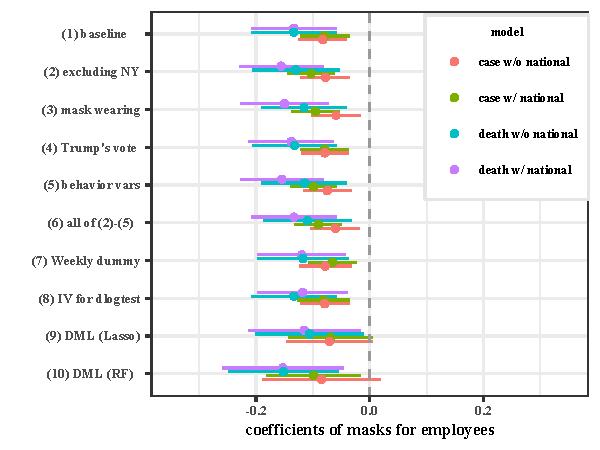
\includegraphics[width=0.5\textwidth]{tables_and_figures/pmaskbus-whisker-14}
      &
      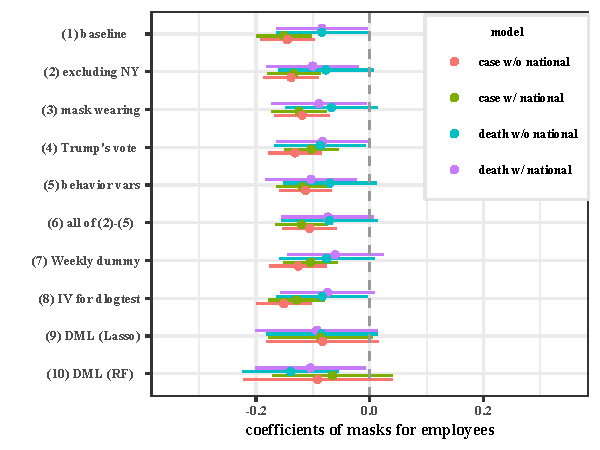
\includegraphics[width=0.5\textwidth]{tables_and_figures/pmaskbus-whisker-7} 
    \end{tabular}
  \end{minipage} \\\smallskip
    \begin{minipage}{\linewidth}
    \centering 
     {\textbf{(B)  closed K-12 Schools}}\\
    \medskip
    \begin{tabular}{cc}  
 $\quad$  (i) baseline timing$^\dagger$ &$\quad$ (ii) alternative timing$^\ddagger$\\ 
      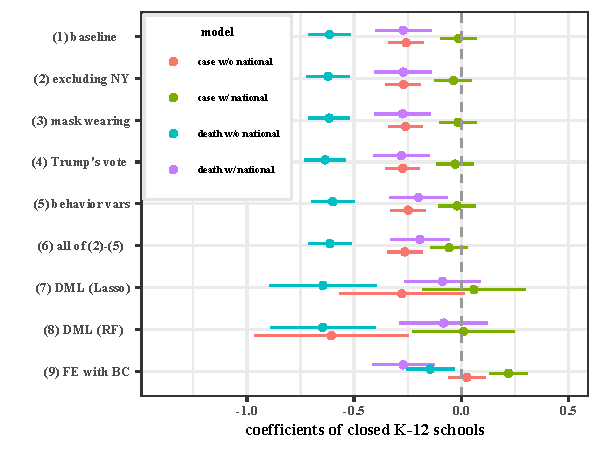
\includegraphics[width=0.5\textwidth]{tables_and_figures/pk12-whisker-14}
      &
      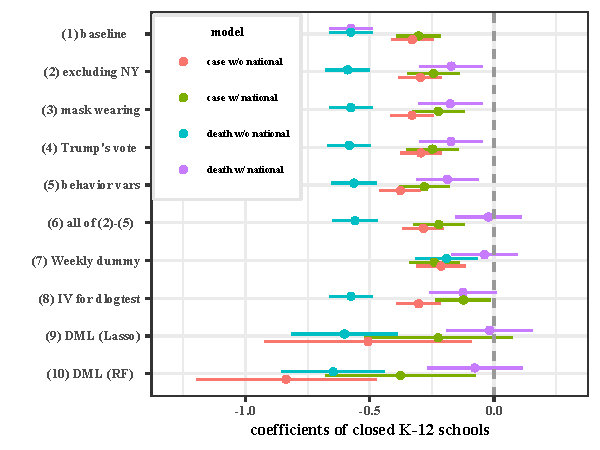
\includegraphics[width=0.5\textwidth]{tables_and_figures/pk12-whisker-7}
          \end{tabular}
  \end{minipage}  
    \begin{flushleft}
      \footnotesize
      $^\dagger$The times from exposure to case confirmation and death reporting  are assumed to be 14 and 21 days, respectively. $^\ddagger$The times from exposure to case confirmation and death reporting  are assumed to be 9 and 24 days, respectively. 
    \end{flushleft}
\end{figure}
   
   \addtocounter{figure}{-1}
\begin{figure}[ht]
  \caption{Estimated Coefficients for Policy Variables:  Sensitivity Analysis (cont.) \label{fig:whisker-2}}\bigskip
  \begin{minipage}{\linewidth}
    \centering
   {\textbf{(C)  stay-at-home orders}}\\
    \medskip
    \begin{tabular}{cc}  
 $\quad$  (i) baseline timing$^\dagger$ &$\quad$ (ii) alternative timing$^\ddagger$\\ 
      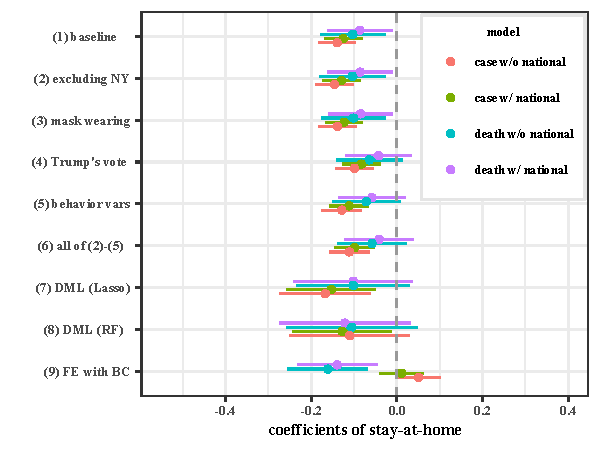
\includegraphics[width=0.5\textwidth]{tables_and_figures/pshelter-whisker-14}
      &
      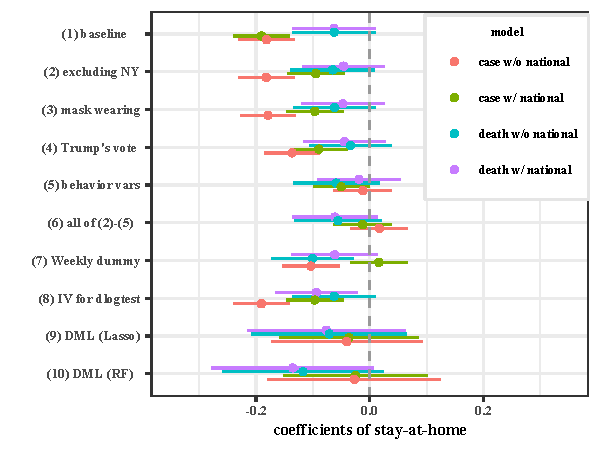
\includegraphics[width=0.5\textwidth]{tables_and_figures/pshelter-whisker-7} 
    \end{tabular}
  \end{minipage} \\ \smallskip
    \begin{minipage}{\linewidth}
    \centering 
     {\textbf{(D)  Average of stay-at-home, closed movie theaters, closed restaurants, and closed  businesses}}\\
    \medskip
    \begin{tabular}{cc}  
 $\quad$  (i) baseline timing$^\dagger$ &$\quad$ (ii) alternative timing$^\ddagger$\\ 
      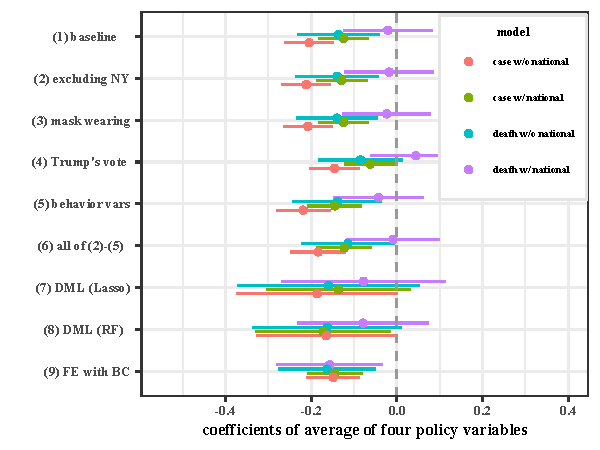
\includegraphics[width=0.5\textwidth]{tables_and_figures/pindex-whisker-14}
      &
      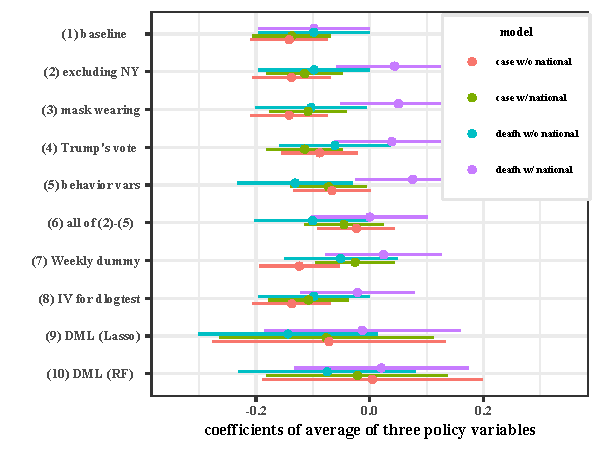
\includegraphics[width=0.5\textwidth]{tables_and_figures/pindex-whisker-7}
          \end{tabular}
  \end{minipage}   
    \begin{flushleft}
      \footnotesize
      $^\dagger$The times from exposure to case confirmation and death reporting  are assumed to be 14 and 21 days, respectively. $^\ddagger$The times from exposure to case confirmation and death reporting  are assumed to be 9 and 24 days, respectively. 
    \end{flushleft}
\end{figure}
   

 \begin{figure}
  \caption{Case and death growth conditional on school closures \label{fig:growthpolicies1}}
  \begin{minipage}{\linewidth}
    \centering
    \begin{tabular}{cc}
       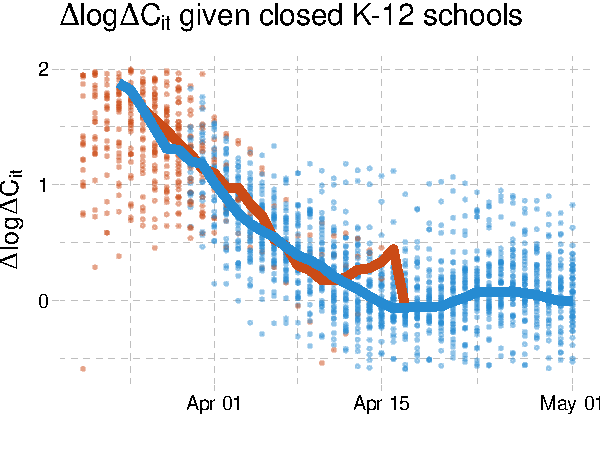
\includegraphics[width=0.483\textwidth]{tables_and_figures/pk12-cases-14}
      &
        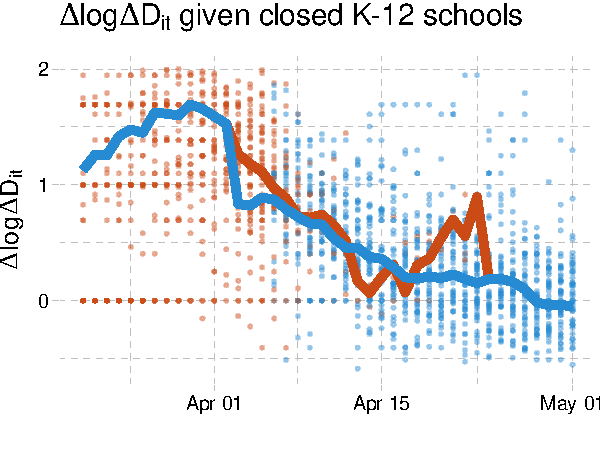
\includegraphics[width=0.483\textwidth]{tables_and_figures/pk12-deaths-21} 
    \end{tabular} 
      \footnotesize In these figures, red points are the case or death
      growth rate in states without each policy 14 (or 21 for deaths)
      days earlier. Blue points are states with each policy 14 (or 21
      for deaths) days earlier. The red line is the average across
      states without each policy. The blue line is the average across
      states with each policy.
  \end{minipage}
\end{figure}




 
%Table \ref{tab:PtoY-robust} presents the regression result for robustness check, where dependent variable is the weekly growth rate of
%  cases  (left panel) or deaths (right panel).   Column (1) replaces four policy variables  (stay-at-home, closure of movie theaters, closure of restaurants, and closure of non-essential businesses) that are highly correlated to each other with the variable of their average values. Column (2) excludes the state of New York, which could be viewed as an outlier in the early pandemic period, from the sample.
% Column (3) adds the percentage of people who wears masks to protect themselves between March 26-April 29, 2020, which controls for people's attitude toward mask wearing in the first half of sample.\footnote{ The survey is conducted online by YouGov and is based on the interviews of 89,347 US adults aged 18 and over between March 26-April 29, 2020.  The survey question is ``Which, if any, of the following measures have you taken in the past 2 weeks to protect yourself from the Coronavirus (COVID-19)?''.}  Column (5) controls for the log of Trump voting shares in 2016 presidential election. Column (6) includes four weeks lagged behavior variables as an additional set of controls; under this specification, our causal interpretation is valid when policy variables are sufficiently random conditional on past behavior variables. Finally, column (6) includes all additional controls in column (3)-(5) using the sample that excludes New York.   The estimated coefficients of mask mandates on case or death growths are significantly negative in all specifications, confirming the importance of mask policy on reducing case and death growths.   
% 
%   
%In Table \ref{tab:PtoY-fe} of the appendix,   we find that the estimated coefficients of mask mandates are significantly negative even when we include state fixed effects. In contrast,  the estimated coefficients of stay-at-home order  and closures of movie theaters, restaurants, and non-essential businesses under fixed effects specification are sometimes different from those under random effects specification, especially when bias correction is applied to the fixed effects estimator.  Non-robustness of the estimated coefficients of these four  policy variables 
% is likely due to high correlations among them (see Table \ref{corr}). In fact, as shown in columns (3)-(4) of Table \ref{tab:PtoY-fe}, the  estimated effects of the average of four policy variables  under fixed effects specification are negative and significant, indicating that  the total effect of four policies is robustly estimated.
%


\subsection{Fixed Effects Regressions (in Appendix)}

Table \ref{tab:PtoY-fe} in the appendix reports the regression result when we include state fixed effects and month dummies. Column (1) reports our baseline estimation when we include state fixed effects while column (2) report the estimate when we apply the bias correction to the fixed effects estimator. Columns (3) and (4) are similar to columns (1) and (2) except that we replace  four policy variables  (stay-at-home, closure of movie theaters, closure of restaurants, and closure of non-essential businesses) with their average values.  Again, the estimated coefficients of mask mandates are significantly negative across different specifications, confirming the importance of mask policy on reducing case and death growths. On the other hand,  the estimated coefficients of stay-at-home order as well as closures of movie theaters, restaurants, and non-essential businesses under fixed effects specification are substantially different from the estimates under random effects specification. This is likely due to muti-colinearity problem as implied by  high correlations among these four policy variables as shown in Table \ref{corr}. When we replace these four policy variables with their average variable in columns (3) and (4), the estimated effect of the sum of four policy variables under fixed effects specification is similar to that under random effects specification in column (1) of Table \ref{tab:PtoY-robust}. 




  \afterpage{
 \begin{landscape}
\begin{table}[!htbp] \centering
 \caption{\label{tab:PtoY-robust}
Sensitivity Check for the Total Effect of Policies on Case and Death Growth ($PI \to Y$)}\vspace{-0.3cm}
 \begin{minipage}{\linewidth}
   \resizebox{\textwidth}{!}{
   \centering
   \tiny
   \begin{tabular}{c|c}
   \begin{minipage}{0.65\linewidth}
     \centering
     \begin{tabular}{@{\extracolsep{1pt}}lcccccc} 
\\[-1.8ex]\hline 
\hline \\[-1.8ex] 
 & \multicolumn{6}{c}{\textit{Dependent variable:}} \\ 
\cline{2-7} 
 & \multicolumn{6}{c}{$\Delta \log \Delta C_{it}$} \\ 
\\[-1.8ex] & (1) & (2) & (3) & (4) & (5) & (6)\\ 
\hline \\[-1.8ex] 
 lag(masks for employees, 14) & $-$0.083$^{**}$ & $-$0.078$^{**}$ & $-$0.059$^{*}$ & $-$0.079$^{**}$ & $-$0.075$^{**}$ & $-$0.060$^{*}$ \\ 
  & (0.038) & (0.039) & (0.031) & (0.034) & (0.035) & (0.035) \\ 
  lag(closed K-12 schools, 14) & $-$0.226$^{**}$ & $-$0.237$^{***}$ & $-$0.229$^{***}$ & $-$0.232$^{***}$ & $-$0.217$^{***}$ & $-$0.223$^{***}$ \\ 
  & (0.089) & (0.092) & (0.086) & (0.075) & (0.083) & (0.068) \\ 
  lag(stay at home, 14) & $-$0.127$^{**}$ & $-$0.132$^{**}$ & $-$0.127$^{**}$ & $-$0.096$^{*}$ & $-$0.110$^{**}$ & $-$0.100$^{*}$ \\ 
  & (0.057) & (0.058) & (0.056) & (0.056) & (0.051) & (0.054) \\ 
  lag(business closure policies, 14) & $-$0.076 & $-$0.077 & $-$0.080 & $-$0.044 & $-$0.095 & $-$0.073 \\ 
  & (0.068) & (0.069) & (0.067) & (0.061) & (0.067) & (0.061) \\ 
  lag(workplaces, 28) &  &  &  &  & $-$0.146 & 0.069 \\ 
  &  &  &  &  & (0.490) & (0.428) \\ 
  lag(retail, 28) &  &  &  &  & $-$0.303 & $-$0.415 \\ 
  &  &  &  &  & (0.356) & (0.358) \\ 
  lag(grocery, 28) &  &  &  &  & $-$0.227 & $-$0.396 \\ 
  &  &  &  &  & (0.250) & (0.255) \\ 
  lag(transit, 28) &  &  &  &  & 0.569$^{*}$ & 0.460 \\ 
  &  &  &  &  & (0.323) & (0.284) \\ 
  lag($\Delta \log \Delta C_{it}$, 14) & 0.040 & 0.034 & 0.038 & 0.042$^{*}$ & 0.042 & 0.044$^{*}$ \\ 
  & (0.024) & (0.024) & (0.024) & (0.024) & (0.028) & (0.026) \\ 
  lag($\log \Delta C_{it}$, 14) & $-$0.137$^{***}$ & $-$0.138$^{***}$ & $-$0.136$^{***}$ & $-$0.155$^{***}$ & $-$0.137$^{***}$ & $-$0.161$^{***}$ \\ 
  & (0.022) & (0.023) & (0.020) & (0.018) & (0.020) & (0.018) \\ 
  $\Delta \log T_{it}$ & 0.156$^{***}$ & 0.143$^{***}$ & 0.158$^{***}$ & 0.148$^{***}$ & 0.147$^{***}$ & 0.120$^{***}$ \\ 
  & (0.044) & (0.042) & (0.044) & (0.044) & (0.046) & (0.044) \\ 
  mask\_percent &  &  & $-$0.656 &  &  & $-$0.487 \\ 
  &  &  & (0.586) &  &  & (0.536) \\ 
  log(Trump voting shares) &  &  &  & 0.323$^{***}$ &  & 0.344$^{***}$ \\ 
  &  &  &  & (0.065) &  & (0.052) \\ 
 \hline \\[-1.8ex] 
state variables & Yes & Yes & Yes & Yes & Yes & Yes \\ 
Month $\times$ state variables & Yes & Yes & Yes & Yes & Yes & Yes \\ 
\hline \\[-1.8ex] 
$\sum_j \mathrm{Policy}_j$ & -0.512$^{***}$ & -0.524$^{***}$ & -0.495$^{***}$ & -0.450$^{***}$ & -0.496$^{***}$ & -0.457$^{***}$ \\ 
 & (0.150) & (0.155) & (0.136) & (0.126) & (0.135) & (0.123) \\ 
Observations & 3,825 & 3,750 & 3,825 & 3,825 & 3,825 & 3,750 \\ 
R$^{2}$ & 0.749 & 0.746 & 0.751 & 0.757 & 0.752 & 0.758 \\ 
Adjusted R$^{2}$ & 0.747 & 0.743 & 0.749 & 0.755 & 0.749 & 0.756 \\ 
\hline 
\hline \\[-1.8ex] 
\textit{Note:}  & \multicolumn{6}{r}{$^{*}$p$<$0.1; $^{**}$p$<$0.05; $^{***}$p$<$0.01} \\ 
\end{tabular} 
   \end{minipage}
     &
   \begin{minipage}{0.65\linewidth}
     \centering
     \begin{tabular}{@{\extracolsep{1pt}}lcccccc} 
\\[-1.8ex]\hline 
\hline \\[-1.8ex] 
 & \multicolumn{6}{c}{\textit{Dependent variable:}} \\ 
\cline{2-7} 
 & \multicolumn{6}{c}{$\Delta \log \Delta D_{it}$} \\ 
\\[-1.8ex] & (1) & (2) & (3) & (4) & (5) & (6)\\ 
\hline \\[-1.8ex] 
 lag(masks for employees, 21) & $-$0.065$^{*}$ & $-$0.062$^{*}$ & $-$0.047 & $-$0.056 & $-$0.061 & $-$0.046 \\ 
  & (0.037) & (0.037) & (0.039) & (0.037) & (0.038) & (0.040) \\ 
  lag(closed K-12 schools, 21) & $-$0.646$^{***}$ & $-$0.649$^{***}$ & $-$0.645$^{***}$ & $-$0.645$^{***}$ & $-$0.618$^{***}$ & $-$0.617$^{***}$ \\ 
  & (0.105) & (0.107) & (0.103) & (0.100) & (0.115) & (0.109) \\ 
  lag(stay at home, 21) & $-$0.006 & $-$0.005 & $-$0.001 & 0.027 & 0.008 & 0.022 \\ 
  & (0.044) & (0.044) & (0.044) & (0.044) & (0.041) & (0.044) \\ 
  lag(business closure policies, 21) & $-$0.108$^{*}$ & $-$0.109$^{*}$ & $-$0.109$^{*}$ & $-$0.062 & $-$0.115$^{*}$ & $-$0.090 \\ 
  & (0.064) & (0.065) & (0.064) & (0.061) & (0.069) & (0.067) \\ 
  lag(workplaces, 35) &  &  &  &  & 1.150$^{**}$ & 1.237$^{**}$ \\ 
  &  &  &  &  & (0.522) & (0.489) \\ 
  lag(retail, 35) &  &  &  &  & $-$0.736$^{**}$ & $-$0.855$^{***}$ \\ 
  &  &  &  &  & (0.358) & (0.328) \\ 
  lag(grocery, 35) &  &  &  &  & 0.137 & $-$0.031 \\ 
  &  &  &  &  & (0.385) & (0.360) \\ 
  lag(transit, 35) &  &  &  &  & 0.033 & $-$0.091 \\ 
  &  &  &  &  & (0.223) & (0.235) \\ 
  lag($\Delta \log \Delta D_{it}$, 21) & 0.031 & 0.028 & 0.031 & 0.035 & 0.014 & 0.025 \\ 
  & (0.034) & (0.036) & (0.034) & (0.034) & (0.039) & (0.042) \\ 
  lag($\log \Delta D_{it}$, 21) & $-$0.077$^{***}$ & $-$0.072$^{***}$ & $-$0.078$^{***}$ & $-$0.095$^{***}$ & $-$0.065$^{***}$ & $-$0.083$^{***}$ \\ 
  & (0.017) & (0.017) & (0.015) & (0.016) & (0.018) & (0.019) \\ 
  mask\_percent &  &  & $-$0.403 &  &  & $-$0.345 \\ 
  &  &  & (0.349) &  &  & (0.351) \\ 
  log(Trump voting shares) &  &  &  & 0.303$^{***}$ &  & 0.296$^{***}$ \\ 
  &  &  &  & (0.066) &  & (0.071) \\ 
 \hline \\[-1.8ex] 
state variables & Yes & Yes & Yes & Yes & Yes & Yes \\ 
Month $\times$ state variables & Yes & Yes & Yes & Yes & Yes & Yes \\ 
\hline \\[-1.8ex] 
$\sum_j \mathrm{Policy}_j$ & -0.825$^{***}$ & -0.826$^{***}$ & -0.802$^{***}$ & -0.736$^{***}$ & -0.786$^{***}$ & -0.731$^{***}$ \\ 
 & (0.114) & (0.115) & (0.107) & (0.109) & (0.127) & (0.124) \\ 
Observations & 4,845 & 4,750 & 4,845 & 4,845 & 4,845 & 4,750 \\ 
R$^{2}$ & 0.441 & 0.433 & 0.442 & 0.448 & 0.444 & 0.442 \\ 
Adjusted R$^{2}$ & 0.437 & 0.429 & 0.438 & 0.444 & 0.440 & 0.437 \\ 
\hline 
\hline \\[-1.8ex] 
\textit{Note:}  & \multicolumn{6}{r}{$^{*}$p$<$0.1; $^{**}$p$<$0.05; $^{***}$p$<$0.01} \\ 
\end{tabular} 
   \end{minipage}

   \end{tabular}
   }
   \begin{flushleft}
     \scriptsize Dependent variable is the weekly growth rate of
     confirmed cases (in the left panel) or deaths (in the right
     panel) as defined in equation (\ref{eq:y}). Columns (2) and (6) exclude the observations of the state of New York.
      The covariates
     include lagged policy variables, which are
     constructed as 7 day moving averages between $t$ to $t-7$ of
     corresponding daily measures.  The row
     ``$\sum_j \mathrm{Policies}_j$'' reports the sum of six policy
     coefficients.  Standard errors are clustered at the state level.
   \end{flushleft}
 \end{minipage}
\end{table}
\end{landscape}
}


  \afterpage{
 \begin{landscape}
\begin{table}[!htbp] \centering
 \caption{\label{tab:PtoY-fe}
Fixed Effects Specification for  the Total Effect of Policies on Case and Death Growth ($PI \to Y$)}\vspace{-0.3cm}
 \begin{minipage}{\linewidth}
   \resizebox{\textwidth}{!}{
   \centering
   \tiny
   \begin{tabular}{c|c}
   \begin{minipage}{0.5\linewidth}
     \centering
     \begin{tabular}{@{\extracolsep{1pt}}lcccccccc} 
\\[-1.8ex]\hline 
\hline \\[-1.8ex] 
 & \multicolumn{8}{c}{\textit{Dependent variable:}} \\ 
\cline{2-9} 
 & \multicolumn{8}{c}{$\Delta \log \Delta C_{it}$} \\ 
\\[-1.8ex] & (1) & (2) & (3) & (4) & (5) & (6) & (7) & (8)\\ 
\hline \\[-1.8ex] 
 lag(masks for employees, 14) & $-$0.114$^{***}$ & $-$0.235$^{***}$ & $-$0.120$^{***}$ & $-$0.209$^{***}$ & $-$0.123$^{***}$ & $-$0.240$^{***}$ & $-$0.132$^{***}$ & $-$0.227$^{***}$ \\ 
  & (0.042) & (0.042) & (0.042) & (0.042) & (0.037) & (0.037) & (0.037) & (0.037) \\ 
  lag(closed K-12 schools, 14) & $-$0.046 & 0.027 & $-$0.001 & 0.085 & 0.084 & 0.221$^{**}$ & 0.139$^{*}$ & 0.313$^{***}$ \\ 
  & (0.079) & (0.079) & (0.068) & (0.068) & (0.084) & (0.084) & (0.074) & (0.074) \\ 
  lag(closed movie theaters, 14) & 0.071 & 0.152$^{**}$ &  &  & 0.059 & 0.112$^{*}$ &  &  \\ 
  & (0.060) & (0.060) &  &  & (0.059) & (0.059) &  &  \\ 
  lag(stay at home, 14) & $-$0.081 & 0.051 &  &  & $-$0.103$^{**}$ & 0.011 &  &  \\ 
  & (0.057) & (0.057) &  &  & (0.049) & (0.049) &  &  \\ 
  lag(closed restaurants, 14) & $-$0.048 & $-$0.121$^{**}$ &  &  & 0.008 & $-$0.016 &  &  \\ 
  & (0.053) & (0.053) &  &  & (0.056) & (0.056) &  &  \\ 
  lag(closed businesses, 14) & $-$0.074 & $-$0.167$^{***}$ &  &  & $-$0.073$^{*}$ & $-$0.168$^{***}$ &  &  \\ 
  & (0.047) & (0.047) &  &  & (0.042) & (0.042) &  &  \\ 
  lag(pindex, 14) &  &  & $-$0.176$^{*}$ & $-$0.149 &  &  & $-$0.163$^{*}$ & $-$0.145 \\ 
  &  &  & (0.094) & (0.094) &  &  & (0.089) & (0.089) \\ 
  lag($\Delta \log \Delta C_{it}$, 14) & 0.028 & $-$0.003 & 0.028 & $-$0.003 & 0.046 & 0.044 & 0.046 & 0.049 \\ 
  & (0.027) & (0.027) & (0.026) & (0.026) & (0.031) & (0.031) & (0.031) & (0.031) \\ 
  lag($\log \Delta C_{it}$, 14) & $-$0.222$^{***}$ & $-$0.178$^{***}$ & $-$0.222$^{***}$ & $-$0.179$^{***}$ & $-$0.195$^{***}$ & $-$0.168$^{***}$ & $-$0.198$^{***}$ & $-$0.171$^{***}$ \\ 
  & (0.018) & (0.018) & (0.017) & (0.017) & (0.025) & (0.025) & (0.025) & (0.025) \\ 
  lag($\Delta \log \Delta C_{it}$.national, 14) &  &  &  &  & $-$0.158$^{***}$ & $-$0.299$^{***}$ & $-$0.147$^{***}$ & $-$0.306$^{***}$ \\ 
  &  &  &  &  & (0.040) & (0.040) & (0.038) & (0.038) \\ 
  lag($\log \Delta C_{it}$.national, 14) &  &  &  &  & $-$0.166$^{***}$ & $-$0.250$^{***}$ & $-$0.158$^{***}$ & $-$0.251$^{***}$ \\ 
  &  &  &  &  & (0.043) & (0.043) & (0.041) & (0.041) \\ 
  $\Delta \log T_{it}$ & 0.113$^{***}$ & 0.173$^{***}$ & 0.108$^{***}$ & 0.168$^{***}$ & 0.118$^{***}$ & 0.177$^{***}$ & 0.112$^{***}$ & 0.173$^{***}$ \\ 
  & (0.039) & (0.039) & (0.040) & (0.040) & (0.037) & (0.037) & (0.038) & (0.038) \\ 
 \hline \\[-1.8ex] 
Observations & 3,624 & 3,624 & 3,624 & 3,624 & 3,624 & 3,624 & 3,624 & 3,624 \\ 
R$^{2}$ & 0.780 & 0.780 & 0.779 & 0.779 & 0.786 & 0.786 & 0.784 & 0.784 \\ 
Adjusted R$^{2}$ & 0.776 & 0.776 & 0.775 & 0.775 & 0.782 & 0.782 & 0.781 & 0.781 \\ 
\hline 
\hline \\[-1.8ex] 
\textit{Note:}  & \multicolumn{8}{r}{$^{*}$p$<$0.1; $^{**}$p$<$0.05; $^{***}$p$<$0.01} \\ 
\end{tabular} 
   \end{minipage}
     &
   \begin{minipage}{0.5\linewidth}
     \centering
     \begin{tabular}{@{\extracolsep{1pt}}lcccc} 
\\[-1.8ex]\hline 
\hline \\[-1.8ex] 
 & \multicolumn{4}{c}{\textit{Dependent variable:}} \\ 
\cline{2-5} 
 & \multicolumn{4}{c}{$\Delta \log \Delta D_{it}$} \\ 
\\[-1.8ex] & (1) & (2) & (3) & (4)\\ 
\hline \\[-1.8ex] 
 lag(masks for employees, 21) & $-$0.047 & $-$0.287$^{**}$ & $-$0.048 & $-$0.279$^{**}$ \\ 
  & (0.044) & (0.131) & (0.045) & (0.111) \\ 
  lag(closed K-12 schools, 21) & $-$0.162$^{*}$ & $-$0.077 & $-$0.172$^{*}$ & $-$0.087 \\ 
  & (0.093) & (0.094) & (0.097) & (0.086) \\ 
  lag(stay at home, 21) & 0.016 & 0.079 & 0.027 & 0.086 \\ 
  & (0.053) & (0.065) & (0.053) & (0.068) \\ 
  lag(business closure policies, 21) & $-$0.113$^{*}$ & $-$0.223$^{***}$ &  &  \\ 
  & (0.062) & (0.076) &  &  \\ 
  lag(closed movie theaters, 21) &  &  & $-$0.013 & $-$0.077 \\ 
  &  &  & (0.060) & (0.057) \\ 
  lag(closed restaurants, 21) &  &  & $-$0.039 & $-$0.056 \\ 
  &  &  & (0.065) & (0.059) \\ 
  lag(closed non-essent bus, 21) &  &  & $-$0.072 & $-$0.105 \\ 
  &  &  & (0.049) & (0.068) \\ 
  lag($\Delta \log \Delta D_{it}$, 21) & 0.051 & 0.045 & 0.051 & 0.045 \\ 
  & (0.034) & (0.041) & (0.034) & (0.039) \\ 
  lag($\log \Delta D_{it}$, 21) & $-$0.129$^{***}$ & $-$0.129$^{***}$ & $-$0.128$^{***}$ & $-$0.189$^{***}$ \\ 
  & (0.015) & (0.015) & (0.015) & (0.024) \\ 
 \hline \\[-1.8ex] 
Observations & 4,845 & 4,845 & 4,845 & 4,845 \\ 
R$^{2}$ & 0.465 & 0.465 & 0.466 & 0.466 \\ 
Adjusted R$^{2}$ & 0.458 & 0.458 & 0.458 & 0.458 \\ 
\hline 
\hline \\[-1.8ex] 
\textit{Note:}  & \multicolumn{4}{r}{$^{*}$p$<$0.1; $^{**}$p$<$0.05; $^{***}$p$<$0.01} \\ 
\end{tabular} 
   \end{minipage}

   \end{tabular}
   }
   \begin{flushleft}
     \scriptsize   All specifications include weekly dummies and state fixed effects. Dependent variable is the weekly growth rate of
     confirmed cases (in the left panel) or deaths (in the right
     panel) as defined in equation (\ref{eq:y}).   Columns (1) and (3) report the standard fixed effects estimator  while Columns (2) and (4) report the fixed effects estimator with bias corrections.    Standard errors are computed by multiplier bootstrap clustered at the state level.
    
   \end{flushleft}
 \end{minipage}
\end{table}
\end{landscape}
}



\begin{footnotesize}

\bibliographystyle{jpe}
\bibliography{covid}

\end{footnotesize}



\end{document}

